\documentclass[compress, 9pt]{beamer}

\def\docroot{../..}

\input{\docroot/../lib/doc/pkg/beamer}
\input{\docroot/../lib/doc/pkg/beamer_flat_style}
\input{\docroot/../lib/doc/math/operators}

\usepackage{array} %% for fixed-width columns in `tabular`

\graphicspath{{\docroot/img/}}

\captionsetup[figure]{labelformat=empty} % remove unnecessary Fig.. prefix.

\title{Скалярное и векторное поля в метрике Шварцшильда}
\author[Василевский~А.В.]{
    Василевский~А.В. \\[\baselineskip]
    {\footnotesize Научный руководитель: Бурланков~Д.Е.}
}
\institute[ННГУ]{Нижегородский университет им. Н.И.~Лобачевского}
\date{2020}

\begin{document}

    \frame[plain]{\titlepage}

    \begin{frame}\frametitle{Введение}

        \begin{itemize}\justifying
            \item Метрика Шварцшильда~--- одна из наиболее фундаментальных метрик в ОТО.
            \item Возникает как результат решения задачи о гравитационном поле в статическом сферически симметричном пространстве.
            \item Велись работы по анализу слабых сферических гравитационных волн (возмущений гравитационного поля) на фоне метрики (= в фоновой метрике) Шварцшильда\nocite{regge_wheeler_1957,Vas2019b}, их взаимодействии с электромагнитным полем.
            \item Нет работ, детально исследующих чисто математически скалярное и векторное (электромагнитное) поля в данной метрике, включая вид сферических гармоник, плотность и потоки энергии.
        \end{itemize}

    \end{frame}

    \begin{frame}\frametitle{Постановка задачи}

        \begin{itemize}\justifying
            \item \textbf{Целью работы} является исследование скалярных и векторных волн (сферических гармоник, плотности и потока энергии) в геометрии Шварцшильда, сравнение их с волнами в плоском пространстве (пространстве Минковского).

            \item Задачи о сферических гармониках скалярного, векторного (электромагнитного) и тензорного (гравитационного) полей объединяются общим алгоритмом решения. Скалярное и векторное поля содержат меньшее число компонент, их проще анализировать.

            \item Здесь в обзорном виде рассматриваются лишь скалярные волны. Векторные волны технически более сложны, однако концептуально не отличаются от скалярных.
        \end{itemize}

    \end{frame}

    \begin{frame}\frametitle{Алгоритм нахождения сферических гармоник}

        Ожидаемый вид гармоник: $h_{lm}$, где $l$,~$m$~--- целые, $-l \le m \le l$, $l \ge 0$.

        \begin{enumerate}\justifying
            \item Составляется лагранжиан поля (скаляр).
            \item Записываются вариационные уравнения.
            \item Методом разделения переменных (Ли-генерации\nocite{burlankov_space_dynamics,BurVas2019}, иным методом) определяется угловая часть гармоник.
            \item Выбирается основная гармоника с $m = 0$.
            \item Для нее решаются вариационные уравнения с известной угловой частью, определяется радиальная.
        \end{enumerate}

    \end{frame}

    \begin{frame}\frametitle{Метрика Шварцшильда}

        Метрика Шварцшильда в сферических координатах $\qty{t,\,r,\,\theta,\,\phi}$~--- диагональная метрика вида
        %
        \begin{equation*}
            g_{\alpha\beta} = \begin{pmatrix}
                -\qty(1 - \frac{r_g}{r}) & 0 & 0 & 0 \\
                0 & \qty(1 - \frac{r_g}{r})^{-1} & 0 & 0 \\
                0 & 0 & r^2 & 0 \\
                0 & 0 & 0 & r^2 \sin^2(\theta)
            \end{pmatrix} .
        \end{equation*}
        %
        Ее детерминант $g = -r^4 \sin^4\theta$, т.е. $\sqrt{-g} = r^2 \sin^2\theta$, как и для плоского пространства в тех же координатах. Здесь $r_g$~--- гравитационный радиус.

    \end{frame}

    \begin{frame}\frametitle{Принцип наименьшего действия}

        Классический лагранжев подход к описанию динамики некоторого поля $f(t,x)$ заключается в сведении физической задачи к задаче минимизации некоторого функционала \textit{действия}\nocite{landau_v1}
        %
        \begin{equation*}
            S\qty[f] = \int\limits_{(1)}^{(2)} L(\vb{x}, \vb{f}(\vb{x}), \vb{f'}(\vb{x})) \dd{\vb{x}}.
        \end{equation*}
        %
        Здесь $\vb{x}$~--- набор из четырех координат, $\vb{f}$, $\vb{f'}$~--- набор из компонент поля.

        В искривленном пространстве $L$ должен быть истинным скаляром, а в результате преобразования координат к нему добавляется якобиан: $L = \mathcal{L} \sqrt{-g}$.

    \end{frame}

    \begin{frame}\frametitle{Тензор энергии-импульса}

        Энергетические характеристики поля определяются его (четырехмерным) тензором энергии-импульса\nocite{landau_v1,landau_v2}:
        %
        \begin{equation*}
            \mathcal{T}_i^k = \sum_s \pdv{f_s}{x^i} \pdv{\mathcal{L}}{\pdv*{f_s}{x^k}} - \delta_i^k \mathcal{L} ,
            \qquad T = \mathcal{T} \sqrt{-g} .
        \end{equation*}

        Компоненты симметричного тензора энергии-импульса определяют скаляр плотности энергии $\epsilon$ и вектор плотности потока энергии $\vb{S}$ поля~$f$:
        %
        \begin{equation*}
            T^{ik} = \begin{pmatrix}
                \epsilon & S^k / c \\
                S^i / c  & \sigma^{ik}
            \end{pmatrix} .
        \end{equation*}

    \end{frame}

    \begin{frame}\frametitle{Скалярное поле}

        \begin{itemize}\justifying
            \item Общий вид скалярной сферической гармоники\nocite{Vas2018a}:
            $$f(t,r,\theta,\phi) = w(r) \exp(-i t) Y_{lm}(\theta,\phi).$$
            Здесь $Y_{lm}$~--- сферические функции.
            \item Лагранжиан и ТЭИ: \begin{gather}
                \mathcal{L} = \frac{1}{2} g^{ij} f_{,i} f_{,j}, \\
                \mathcal{T}_{ij} = \frac{1}{2} \qty(- g_{ij} f^{,s} f_{,s} + 2 f_{,i} f_{,j}).
            \end{gather}
            (Здесь и далее \enquote{${}_{,k}$} обозначает производную по $x^k$.)
        \end{itemize}

    \end{frame}

    \begin{frame}\frametitle{Скалярное поле в плоском пространстве}

        \begin{itemize}\justifying
            \item В плоском пространстве $g = \mathop{\mathrm{diag}}(-1, 1, 1, 1)$~--- метрика Минковского.
            \item Вариационное уравнение дает ДУ для радиальной части:
            \begin{equation*}
                r^2 w''(r) + 2 r w'(r) + (l\,(l+1) - r^2) w(r) = 0.
            \end{equation*}
            \item Его решение~--- сферические функции Бесселя $j_l(r)$, $y_l(r)$ (действительные; стоячие волны) или сферические функции Ганкеля $h_{1,2}(r) = j_l(r) \pm i y_l(r)$ (комплексные; бегущие волны).
        \end{itemize}
        %
        \begin{figure}[h]
            \centering
            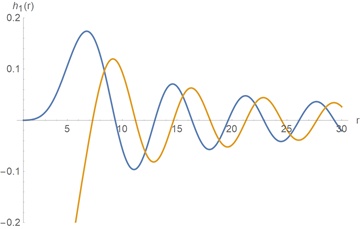
\includegraphics[width=0.45\textwidth]{scal-vec/scal-h1}\hspace{8pt}%
            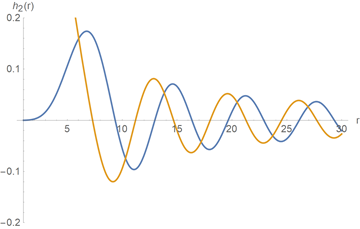
\includegraphics[width=0.45\textwidth]{scal-vec/scal-h2}\hspace{8pt}%
            \caption[]{Бегущие волны, $l = 5$}%
        \end{figure}

    \end{frame}

    \begin{frame}\frametitle{Скалярное поле в плоском пространстве (энергия)}

        \begin{itemize}\justifying
            \item Рассматриваются только средние по периоду характеристики.
            \item Поток энергии либо отсутствует (стоячие волны), либо константа (бегущие волны).
        \end{itemize}
        %
        \begin{figure}[h]
            \centering
            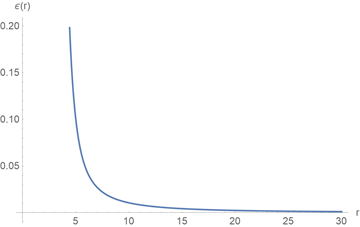
\includegraphics[width=0.35\textwidth]{scal-vec/scal-h1-ee-p2}\hspace{8pt}%
            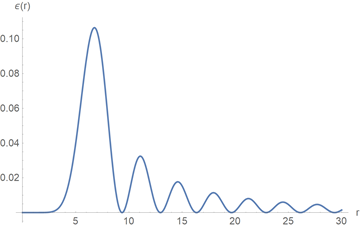
\includegraphics[width=0.35\textwidth]{scal-vec/scal-j1-ee-p2}\hspace{8pt}%
            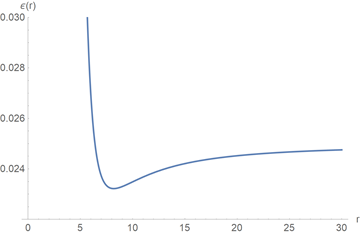
\includegraphics[width=0.35\textwidth]{scal-vec/scal-h1-ee}\hspace{8pt}%
            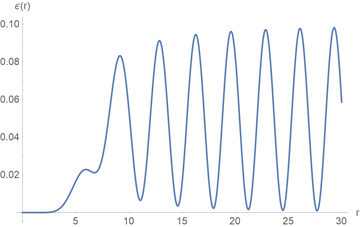
\includegraphics[width=0.35\textwidth]{scal-vec/scal-j1-ee}\hspace{8pt}%
            \caption[]{Плотность энергии $l=5$ моды бегущей (слева) и стоячей справа) волн в зависимости от радиуса при фиксированных направлениях $\theta = \pi/2$ и $\theta = \pi/4$}%
        \end{figure}

    \end{frame}

    \begin{frame}\frametitle{Скалярное поле в метрике Шварцшильда}

        \begin{itemize}\justifying
            \item Вариационное уравнение сводится к сложному ДУ:
            \begin{equation*}
                w''(r) + \qty(\frac{1}{r} + \frac{1}{r - r_g})\, w'(r) - \qty(\frac{l\,(l+1)}{r\, (r-r_g)} - \frac{r^2}{(r-r_g)^2})\, w(r) = 0.
            \end{equation*}
            \item Оно не имеет простого решения в виде известных специальных функций.
            \item Решение можно получить в виде ряда в окрестности регулярной особой точки\nocite{whittaker_watson_1, fedoryuk_de} $r = r_g$ с радиусом сходимости $r_g$.
            \item Распространение на $r \gg r_g$ можно произвести численно. Начальные условия для численного решения можно получить, вычислив ряд в некоторой точке $r^* \in (r_g,\ 2\, r_g)$.
            \item Особенность $r = r_g$ сказывается на структуре решений существенно. Пространство делится на две области: $r < r_g$ и $r > r_g$. Свойства волн в каждой из областей различны.
        \end{itemize}

    \end{frame}

    \begin{frame}

        \begin{figure}[h]
            \centering
            %
            \subfloat[][]{%
                \label{fig:scal-rg-sec1}%
                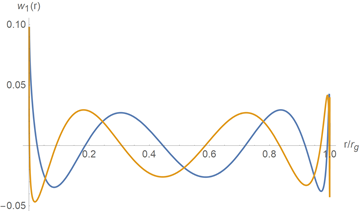
\includegraphics[width=0.45\textwidth]{scal-vec/scal-rg-sec1}}%
            \hspace{8pt}%
            %
            \subfloat[][]{%
                \label{fig:scal-rg-sec2}%
                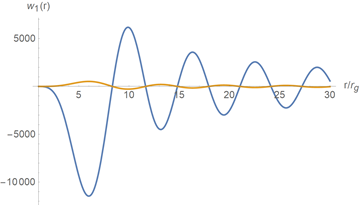
\includegraphics[width=0.45\textwidth]{scal-vec/scal-rg-sec2}}%
            \hspace{8pt}%
            %
            \subfloat[][]{%
                \label{fig:scal-rg-sec1-rg}%
                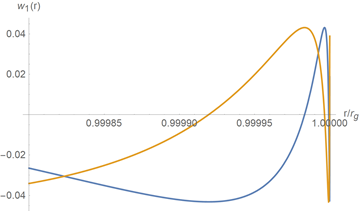
\includegraphics[width=0.45\textwidth]{scal-vec/scal-rg-sec1-rg}}%
            \hspace{8pt}%
            %
            \subfloat[][]{%
                \label{fig:scal-rg-sec2-rg}%
                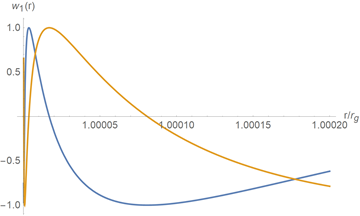
\includegraphics[width=0.45\textwidth]{scal-vec/scal-rg-sec2-rg}}%
            \hspace{8pt}%
            %
            \caption[]{Решение $w_1(r)$ ($l = 5$, действительная и мнимая части) в различных областях:
                \subref{fig:scal-rg-sec1}~$r<r_g$,
                \subref{fig:scal-rg-sec2}~$r > r_g$,
                \subref{fig:scal-rg-sec1-rg}~$r = r_g - \varepsilon$,
                \subref{fig:scal-rg-sec2-rg}~$r = r_g + \varepsilon$}%
            \label{fig:scal-rg}%
        \end{figure}

    \end{frame}

    \begin{frame}
        %
        \begin{figure}[h]
            \centering
            %
            \subfloat[][]{%
                \label{fig:scal-rg2-sec1}%
                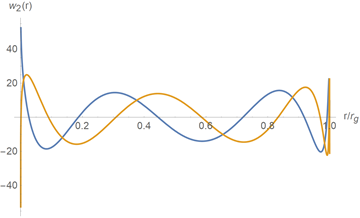
\includegraphics[width=0.45\textwidth]{scal-vec/scal-rg2-sec1}}%
            \hspace{8pt}%
            %
            \subfloat[][]{%
                \label{fig:scal-rg2-sec2}%
                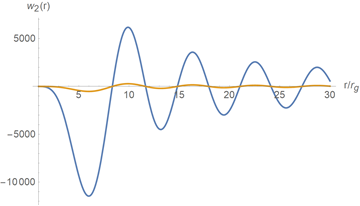
\includegraphics[width=0.45\textwidth]{scal-vec/scal-rg2-sec2}}%
            \hspace{8pt}%
            %
            \subfloat[][]{%
                \label{fig:scal-rg2-sec1-rg}%
                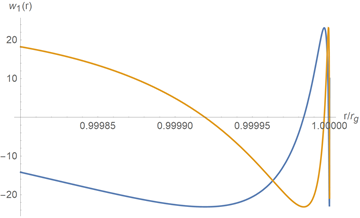
\includegraphics[width=0.45\textwidth]{scal-vec/scal-rg2-sec1-rg}}%
            \hspace{8pt}%
            %
            \subfloat[][]{%
                \label{fig:scal-rg2-sec2-rg}%
                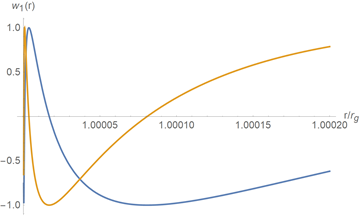
\includegraphics[width=0.45\textwidth]{scal-vec/scal-rg2-sec2-rg}}%
            \hspace{8pt}%
            %
            \caption[]{Решение $w_2(r)$ ($l = 5$, действительная и мнимая части) в различных областях:
                \subref{fig:scal-rg2-sec1}~$r<r_g$,
                \subref{fig:scal-rg2-sec2}~$r > r_g$,
                \subref{fig:scal-rg2-sec1-rg}~$r = r_g - \varepsilon$,
                \subref{fig:scal-rg2-sec2-rg}~$r = r_g + \varepsilon$}%
            \label{fig:scal-rg2}%
        \end{figure}

    \end{frame}

    \begin{frame}\frametitle{Скалярное поле в метрике Шварцшильда}

        \begin{itemize}\justifying
            \item Пространство делится на две области, плюс одну общую подобласть.
            \item При $r < r_g$ волны бегущие (можно обратить в стоячие). Действительная и мнимая части ортогональны. Два решения различаются лишь знаком мнимой части и масштабом.
            \item При $r \gg r_g$ волны (почти) стоячие. Действительная и мнимая части отличаются лишь амплитудой. Два решения отличаются лишь знаком мнимой части. Волны нельзя сделать бегущими.
            \item При $r \to r_g$ частота волн бесконечно возрастает. Волны бегущие (нельзя сделать стоячими сразу при $r < r_g$ и $r > r_g$). Шварцшильдовский радиус $r_g$ является горизонтом событий~--- данной фиксированной точке волны потребуется бесконечное время на его преодоление. Плотность энергии здесь неограниченно возрастает.
        \end{itemize}

    \end{frame}

    \begin{frame}
        %
        \begin{figure}[h]
            \centering
            %
            \subfloat[][]{%
                \label{fig:scal-rg-ee-sec1}%
                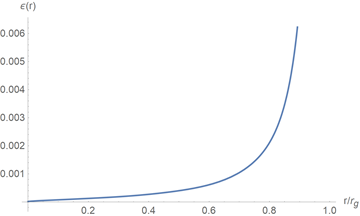
\includegraphics[width=0.30\textwidth]{scal-vec/scal-rg-ee-sec1}}%
            \hspace{8pt}%
            %
            \subfloat[][]{%
                \label{fig:scal-rg-ee-sec2-rg}%
                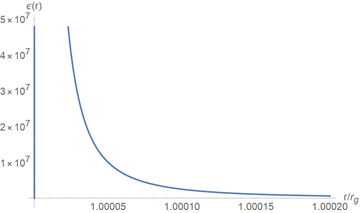
\includegraphics[width=0.30\textwidth]{scal-vec/scal-rg-ee-sec2-rg}}%
            \hspace{8pt}%
            %
            \subfloat[][]{%
                \label{fig:scal-rg-ee-sec2}%
                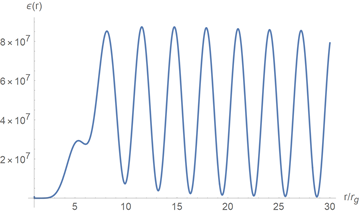
\includegraphics[width=0.30\textwidth]{scal-vec/scal-rg-ee-sec2}}%
            \hspace{8pt}%
            %
            \subfloat[][]{%
                \label{fig:scal-rg-uu-sec1}%
                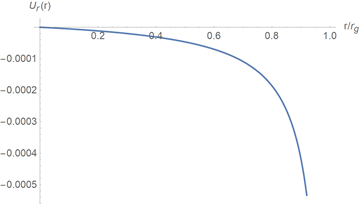
\includegraphics[width=0.30\textwidth]{scal-vec/scal-rg-uu-sec1}}%
            \hspace{8pt}%
            %
            \subfloat[][]{%
                \label{fig:scal-rg-uu-sec2-rg}%
                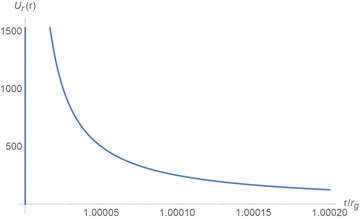
\includegraphics[width=0.30\textwidth]{scal-vec/scal-rg-uu-sec2-rg}}%
            \hspace{8pt}%
            %
            \subfloat[][]{%
                \label{fig:scal-rg-uu-sec2}%
                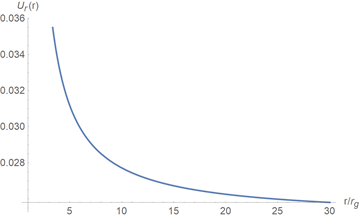
\includegraphics[width=0.30\textwidth]{scal-vec/scal-rg-uu-sec2}}%
            \hspace{8pt}%
            %
            \caption[]{Плотность (сверху) и поток энергии (радиальная компонента; снизу) $l=5$ моды первого бегущего решения в зависимости от радиуса в различных областях пространства при фиксированном угле $\theta = \pi/4$}%
            \label{fig:scal-ee-uu}%
        \end{figure}

    \end{frame}

    \begin{frame}
        %
        \begin{figure}[h]
            \centering
            %
            \subfloat[][]{%
                \label{fig:scal-rg-ee-sec2-p2}%
                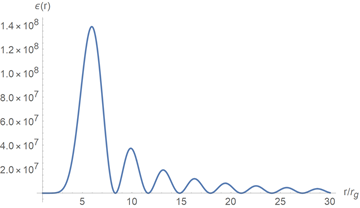
\includegraphics[width=0.45\textwidth]{scal-vec/scal-rg-ee-sec2-p2}}%
            \hspace{8pt}%
            %
            \subfloat[][]{%
                \label{fig:scal-rg-uu-sec2-p2}%
                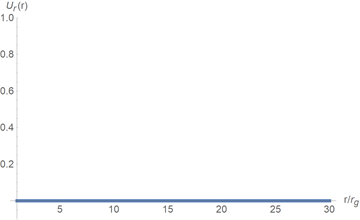
\includegraphics[width=0.45\textwidth]{scal-vec/scal-rg-uu-sec2-p2}}%
            \hspace{8pt}
            %
            \caption[]{Плотность \subref{fig:scal-rg-ee-sec2-p2} и поток энергии (радиальная компонента) \subref{fig:scal-rg-uu-sec2-p2} $l=5$ моды первого бегущего решения в зависимости от радиуса в области $r \gg r_g$ при фиксированном угле $\theta = \pi/2$. Поток энергии здесь полностью отсутствует~--- волны в данном направлении чисто стоячие}%
            \label{fig:scal-ee-uu-p2}%
        \end{figure}

    \end{frame}

    \begin{frame}\frametitle{Векторное поле}

        \begin{itemize}\justifying
            \item Концептуально результаты не отличаются от результатов для скалярного поля.
            \item Справедливы те же замечания относительно бегущих и стоячих волн в различных областях пространства.
            \item При приближении к горизонту событий $r_g$ скалярные и векторные волны ведут себя одинаково.
            \item Плотность и потоки энергии векторных волн в плоском и искривленном пространстве соотносятся также, как и у скалярных волн.
        \end{itemize}

    \end{frame}

    \begin{frame}\frametitle{Анализ решений}

        \begin{itemize}\justifying
            \item В метрике Шварцшильда существенно меняется характер сферических гармоник тех или иных волн ввиду наличия особенности самой метрики~--- гравитационного радиуса~--- который делит пространство на две части: внутреннюю область (\enquote{под} гравитационным радиусом) и внешнюю область (\enquote{над} гравитационным радиусом).
            \item  Имеет место смешанный характер самих волн: будучи бегущими в одной области пространства, они остаются стоячими в другой. Нельзя получить чисто бегущие волны над гравитационным радиусом. Нельзя получить чисто стоячие решения во всем пространстве.
            \item  Имеет место нарастание частоты волн при приближении к гравитационному радиусу. Данной точке волны потребуется бесконечно большое время для пересечения горизонта событий.
            \item Исследование поведения волны в координатах, не содержащих особенности на гравитационном радиусе, представляет большой интерес, однако выходит за рамки данной работы.
        \end{itemize}

    \end{frame}

    \begin{frame}\frametitle{Выводы}

        \begin{itemize}\justifying
            \item Построены сферические гармоники скалярных и векторных волн в метрике Шварцшильда.
            \item Обозначены особенности данных волн относительно волн в плоском пространстве.
            \item Описаны энергетические характеристики волн (плотность, поток энергии).
            \item Имеются дополнительные направления для исследования (волны в глобальном времени\nocite{burlankov_space_dynamics}, получение точного аналитического решения, волны в координатах без особенности на гравитационном радиусе).
        \end{itemize}

    \end{frame}

    \begin{frame}\frametitle{Литература}

        {\tiny{
        \bibliographystyle{\docroot/../lib/doc/bib/utf8gosttu}
        \bibliography{\docroot/../lib/doc/bib/math,\docroot/../lib/doc/bib/physics}
        }}

    \end{frame}

\end{document}
